\documentclass{article}
\usepackage{graphicx}
\usepackage[top=1in, bottom=1in, left=1in, right=1in]{geometry}

\begin{document}

\title{Text Technologies for Data Science: Assessment 2}
\author{s1107496}

\maketitle

\section{Introduction}
This report describes the implementation of two information retrieval algorithms, brute.py and index.py, as well as refinements to the latter as implemented in best.py.

\section{brute.py and index.py}
\subsection{brute.py}
In brute.py, each news story was first transformed to lowercase and tokenized on whitespace, following which the tf-idf weighted cosine denominator component for the story was computed. Then, for every prior story, the tf-idf weighted cosine was calculated, drawing from both a pre-computed dictionary of token idf scores and a list-based cache of tokenized story/tf-idf weighted cosine denominator component tuples. In this way, only the query-document-unique numerator of the tf-idf weighted cosine formula needed to be calculated (for all tokens in both the query and document).  If the score of the best matching document exceeded the given threshold, the result was written to a file and immediately flushed. Finally, the token/denominator tuple for the latest news story was added to the aforementioned cache.
\subsection{index.py}
index.py improved upon brute.py by implementing a term-at-a-time indexing. The index was represented as a dictionary with tokens as keys and lists of story number/token count tuples as values. As in brute.py, tf-idf weighted cosine denominators were also cached for each story. When calculating tf-idf weighted cosine, partial story scores were stored in a dictionary. For 10,000 stories, index.py ran roughly 3.8 times faster than brute.py.

\section{best.py}
best.py included a number of refinements over index.py, as listed below. For 10,000 stories, best.py ran 18.7 times faster than index.py (71.4 times faster than brute.py). As measured against the provided pairs.ref, best.py had an accuracy of 91.13\%.
\subsection{Stop word removal}
After initial tokenization, all tokens from the English-language stop word list provided by \texttt{nltk} were removed. Additionally, domain-specific stop words (where idf < 3.38211) were removed. This increased speed by 934\% (measured on 10,000 stories), while lowering accuracy by 8.87\%. An additional speed improvement of 9.5\% could have been made at the expense of a further 0.78\% loss of accuracy, but this was deemed too likely to result in overfitting stop words to the given data.
\subsection{Identical story checking}
A large number of stories in news.txt had duplicates, the earliest of which would always be the best match for that story. Taking advantage of this, directly following tokenization, the first 40 tokens were checked against a cache. In the event of a hit, the associated value (representing the first seen instance of the story) was immediately output, and the story was not added to the index. Otherwise, a new entry in the cache was made for the story, and processing continued as normal. This increased processing speed by 83\%.
\subsection{Pre-calculation of token idf}
Following tokenization, a sparse representation of the story was created using token counts multiplied by token idf, as opposed to raw token counts. This increased processing speed by 15\%.
\subsection{Python-specific improvements}
A number of small Python-specific efficiency improvements were made, each of which had a marginal positive effect on speed. These included using \texttt{frozenset} instead of \texttt{list} where appropriate, directly calling magic methods (e.g. \texttt{obj.\_\_contains\_\_(x)} instead of \texttt{x in obj}), and moving object dictionary accesses (such as \texttt{file.write}, \texttt{dict.get}) outside of loops (where possible).

\section{Comparison of algorithm running times}
Tests were run on a DICE machine with an i5 processor and 8GB RAM.
\begin{figure}[ht!]
\centering
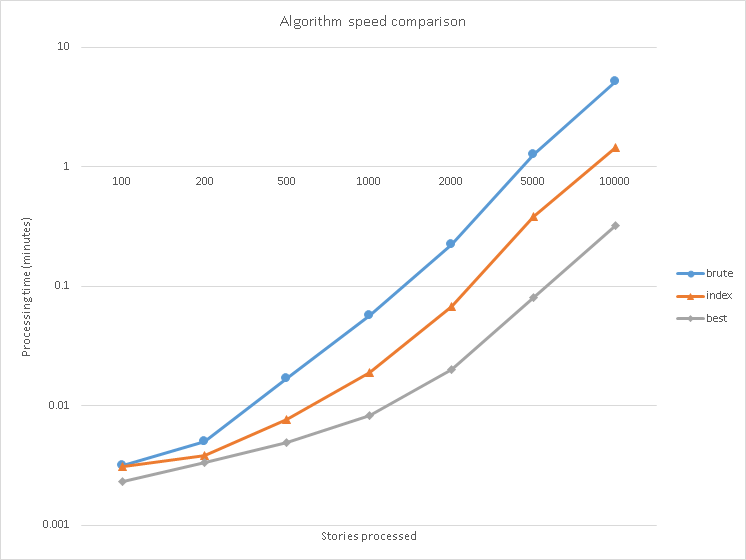
\includegraphics[width=165mm]{algos2.png}
\end{figure}


\end{document}